\documentclass{article}
\usepackage[utf8]{inputenc}
\usepackage{graphicx}
\graphicspath{ {images/} }
\usepackage{algorithm,algorithmic}
\usepackage{amsmath}
\usepackage{amssymb}
\usepackage{mathtools}


\title{GPU based optimizations for large graph adjacency matrices}
\author{Sanjana Garg, 13617}
\date{28 April, 2017}

\begin{document}

\maketitle

\section*{Introduction}
BitMat is a novel compressed bit-vector based index structure previously developed for efficient storage of RDF graph's adjacency matrices. It stores the RDF triples using a 3-dimensional bit-matrix where the three dimensions are subject, object and predicate. A bit is set to $1$ in this matrix if that triple is present. Since, this matrix is sparse, these mats are stored in a compresses format following the D-gap compression scheme.\\

\section*{Motivation}
Fold and unfold are the two primitives in the BitMat system heavily used in the pattern queries for fast operations on the compressed matrices without uncompressing them. Fold and unfold operations operate on each compressed row in a "mutually exclusive" manner using mask bit-vectors (generated by pattern match queries). In this regard, the main contribution of this project is to exploit the "mutual exclusivity" of these operations using the parallelization offered by the GPUs. 

\section*{Fold operation}
The fold operation performs an \textbf{OR} operation over all the rows/columns to give a folded array of the column/row dimension.
Consider an uncompressed bitmat of the following form. Here, the matrix represents the bitmat and the array below that represents the folded array.

\begin{algorithm}[H]
      \begin{algorithmic}[1]
        \FOR {\texttt{(i=0 ; i<n; i++)}}
            \FOR{\texttt{(j=0 ; j<m; j++)}}
                \STATE $foldarr[j] \gets foldarr[j]$ or $BitMat[i][j]$
            \ENDFOR
        \ENDFOR
      \end{algorithmic}
      \caption{CPU\_Fold(BitMat, n, m)}
\end{algorithm}


\begin{figure}[ht]
        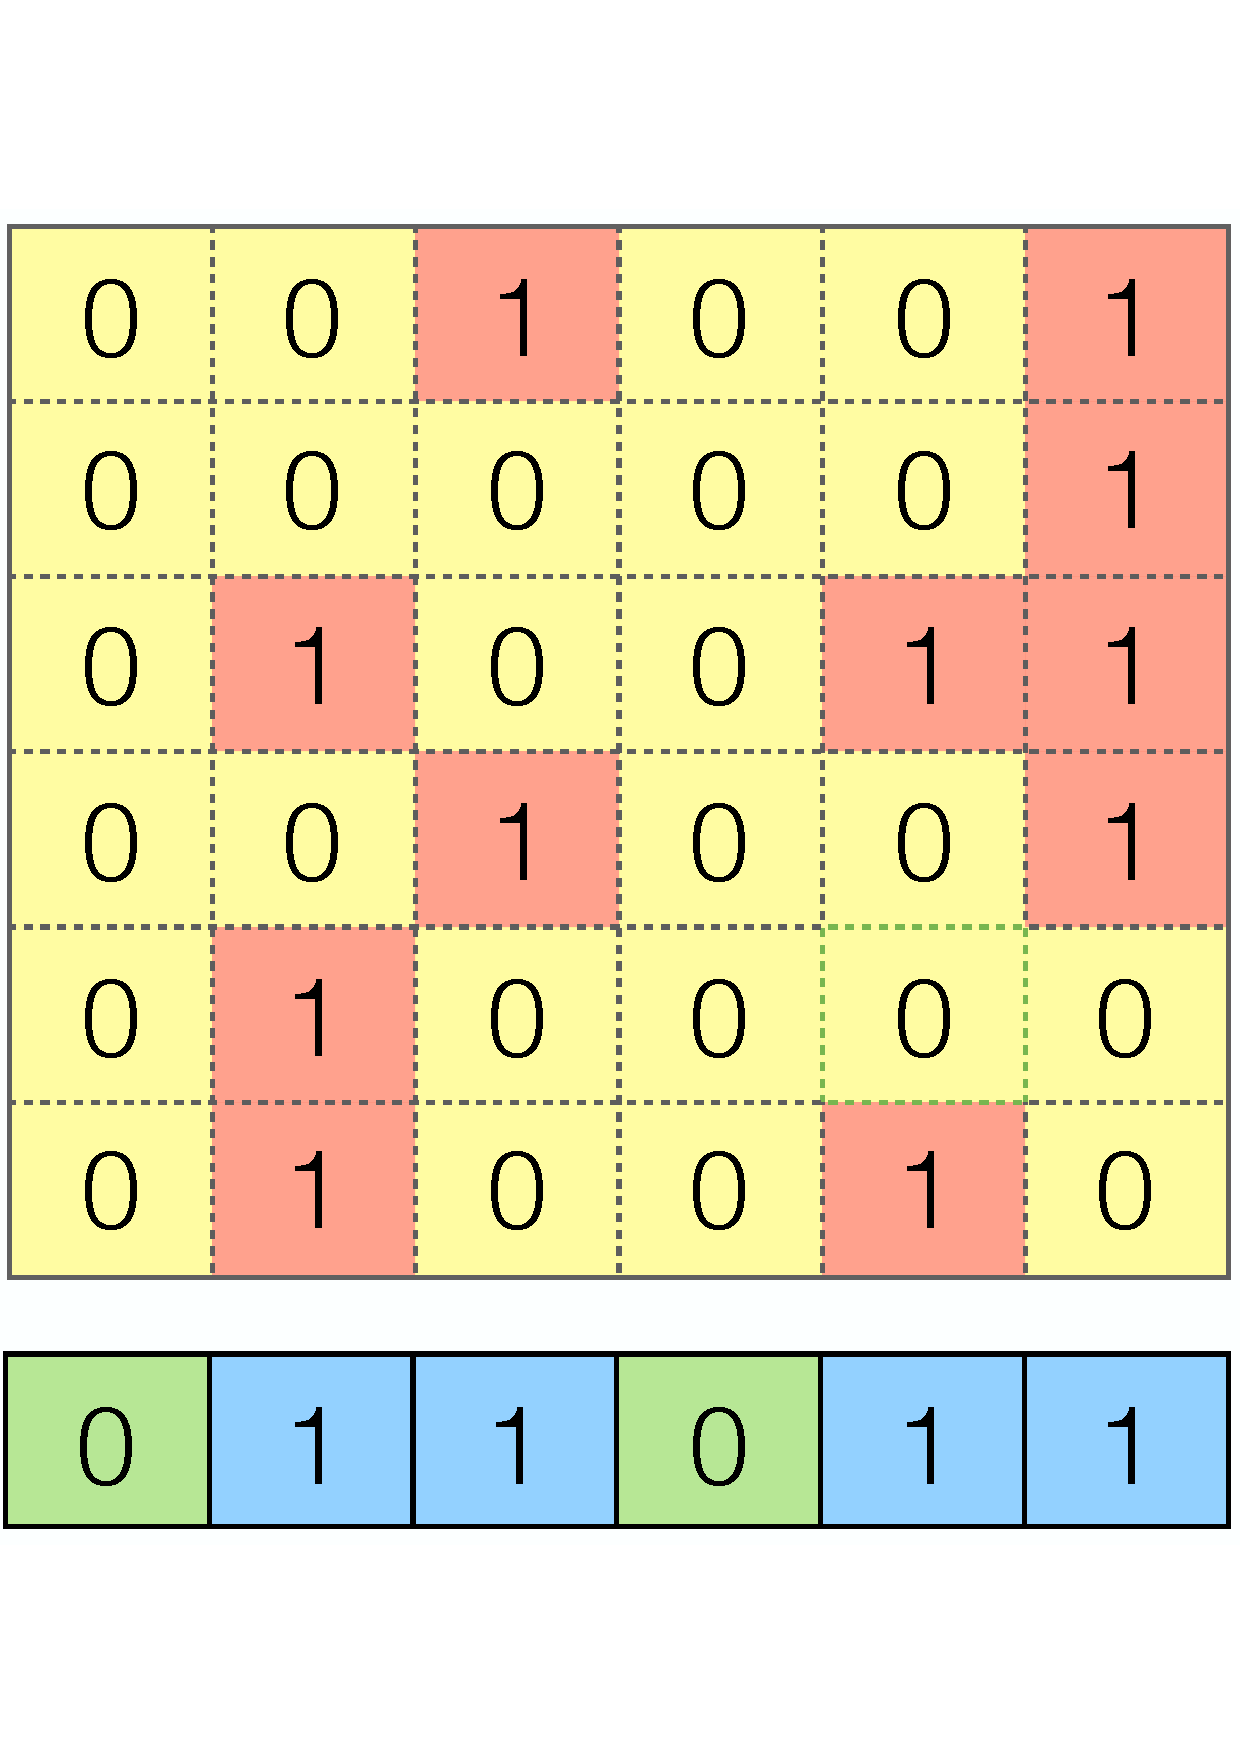
\includegraphics[width=.5\textwidth]{OR.pdf}
        \caption{In this figure, matrix represents an uncompressed BitMat while the array represents the folded array. }
        \centering
\end{figure}

\section*{Unfold operation}
The unfold operation takes as input a bitmat and a mask array and outputs a bitmat with all it's rows ANDed with the mask array.

\begin{algorithm}[H]
      \begin{algorithmic}[1]
        \FOR {\texttt{(i=0; i<n; i++)}}
            \FOR{\texttt{(j=0; j<m; j++)}}
                \STATE $output[i][j] \gets maskarr[j] \& input[i][j]$
            \ENDFOR
        \ENDFOR
      \end{algorithmic}
      \caption{CPU\_Fold(input, maskarr, output, n, m)}
\end{algorithm}

\begin{figure}[ht]
        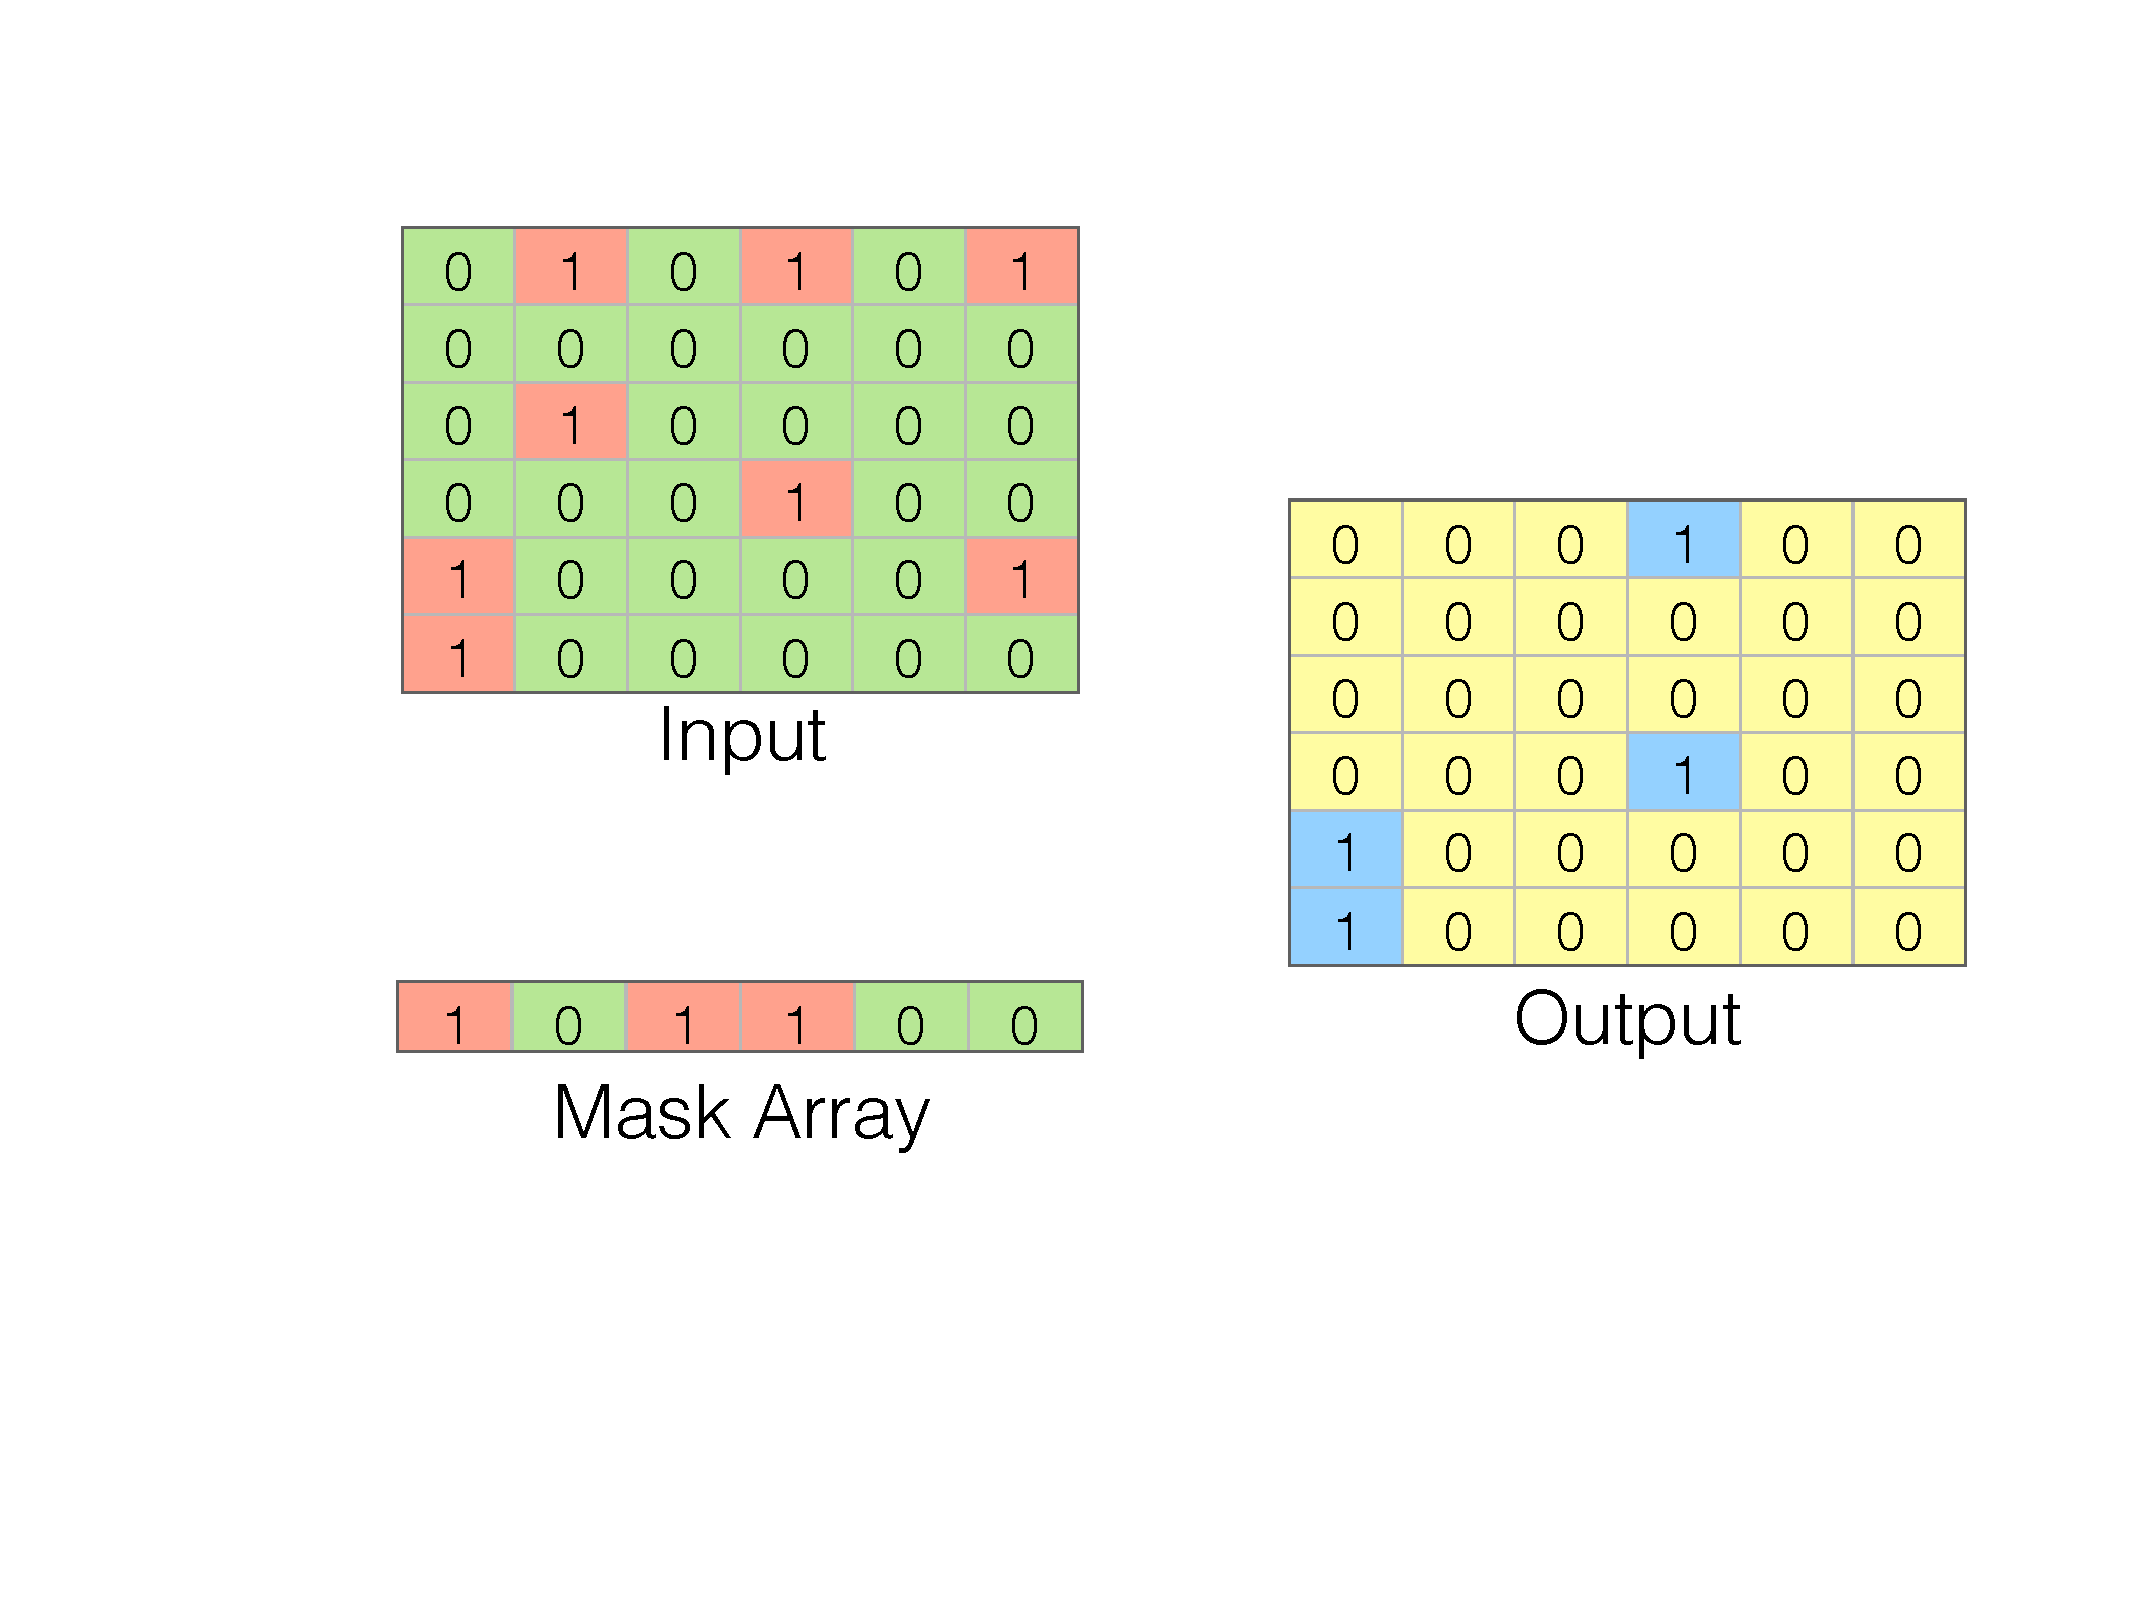
\includegraphics[width=\textwidth]{AND.pdf}
        \caption{In this figure, matrix represents an uncompressed BitMat while the array represents the mask array. Output is the result of applying unfold operation on input as outlined in the algorithm above}
        \centering
\end{figure}

\section*{Parallelization in CUDA}
\subsection*{Architecture}
CUDA is a library developed to exploit the parallelization in GPUs. The architecture divides the code and data into two parts: device and host. Here device, refers to the GPU and host to the CPU machine. The parallelization is performed by threads. The threads are organized into blocks where a block is executed by a multiprocessing unit. The blocks are further organized into a grid. Both the threads and blocks can have a 1, 2 or 3-dimensional index. The grids map to GPUs, blocks to multiprocessors and threads to stream processors.\\

In this project, I have used a 1-dimensional indexing for both threads and blocks as the parallelization is only on 1-dimension int the BitMat, either row or column.

\begin{figure}[ht]
        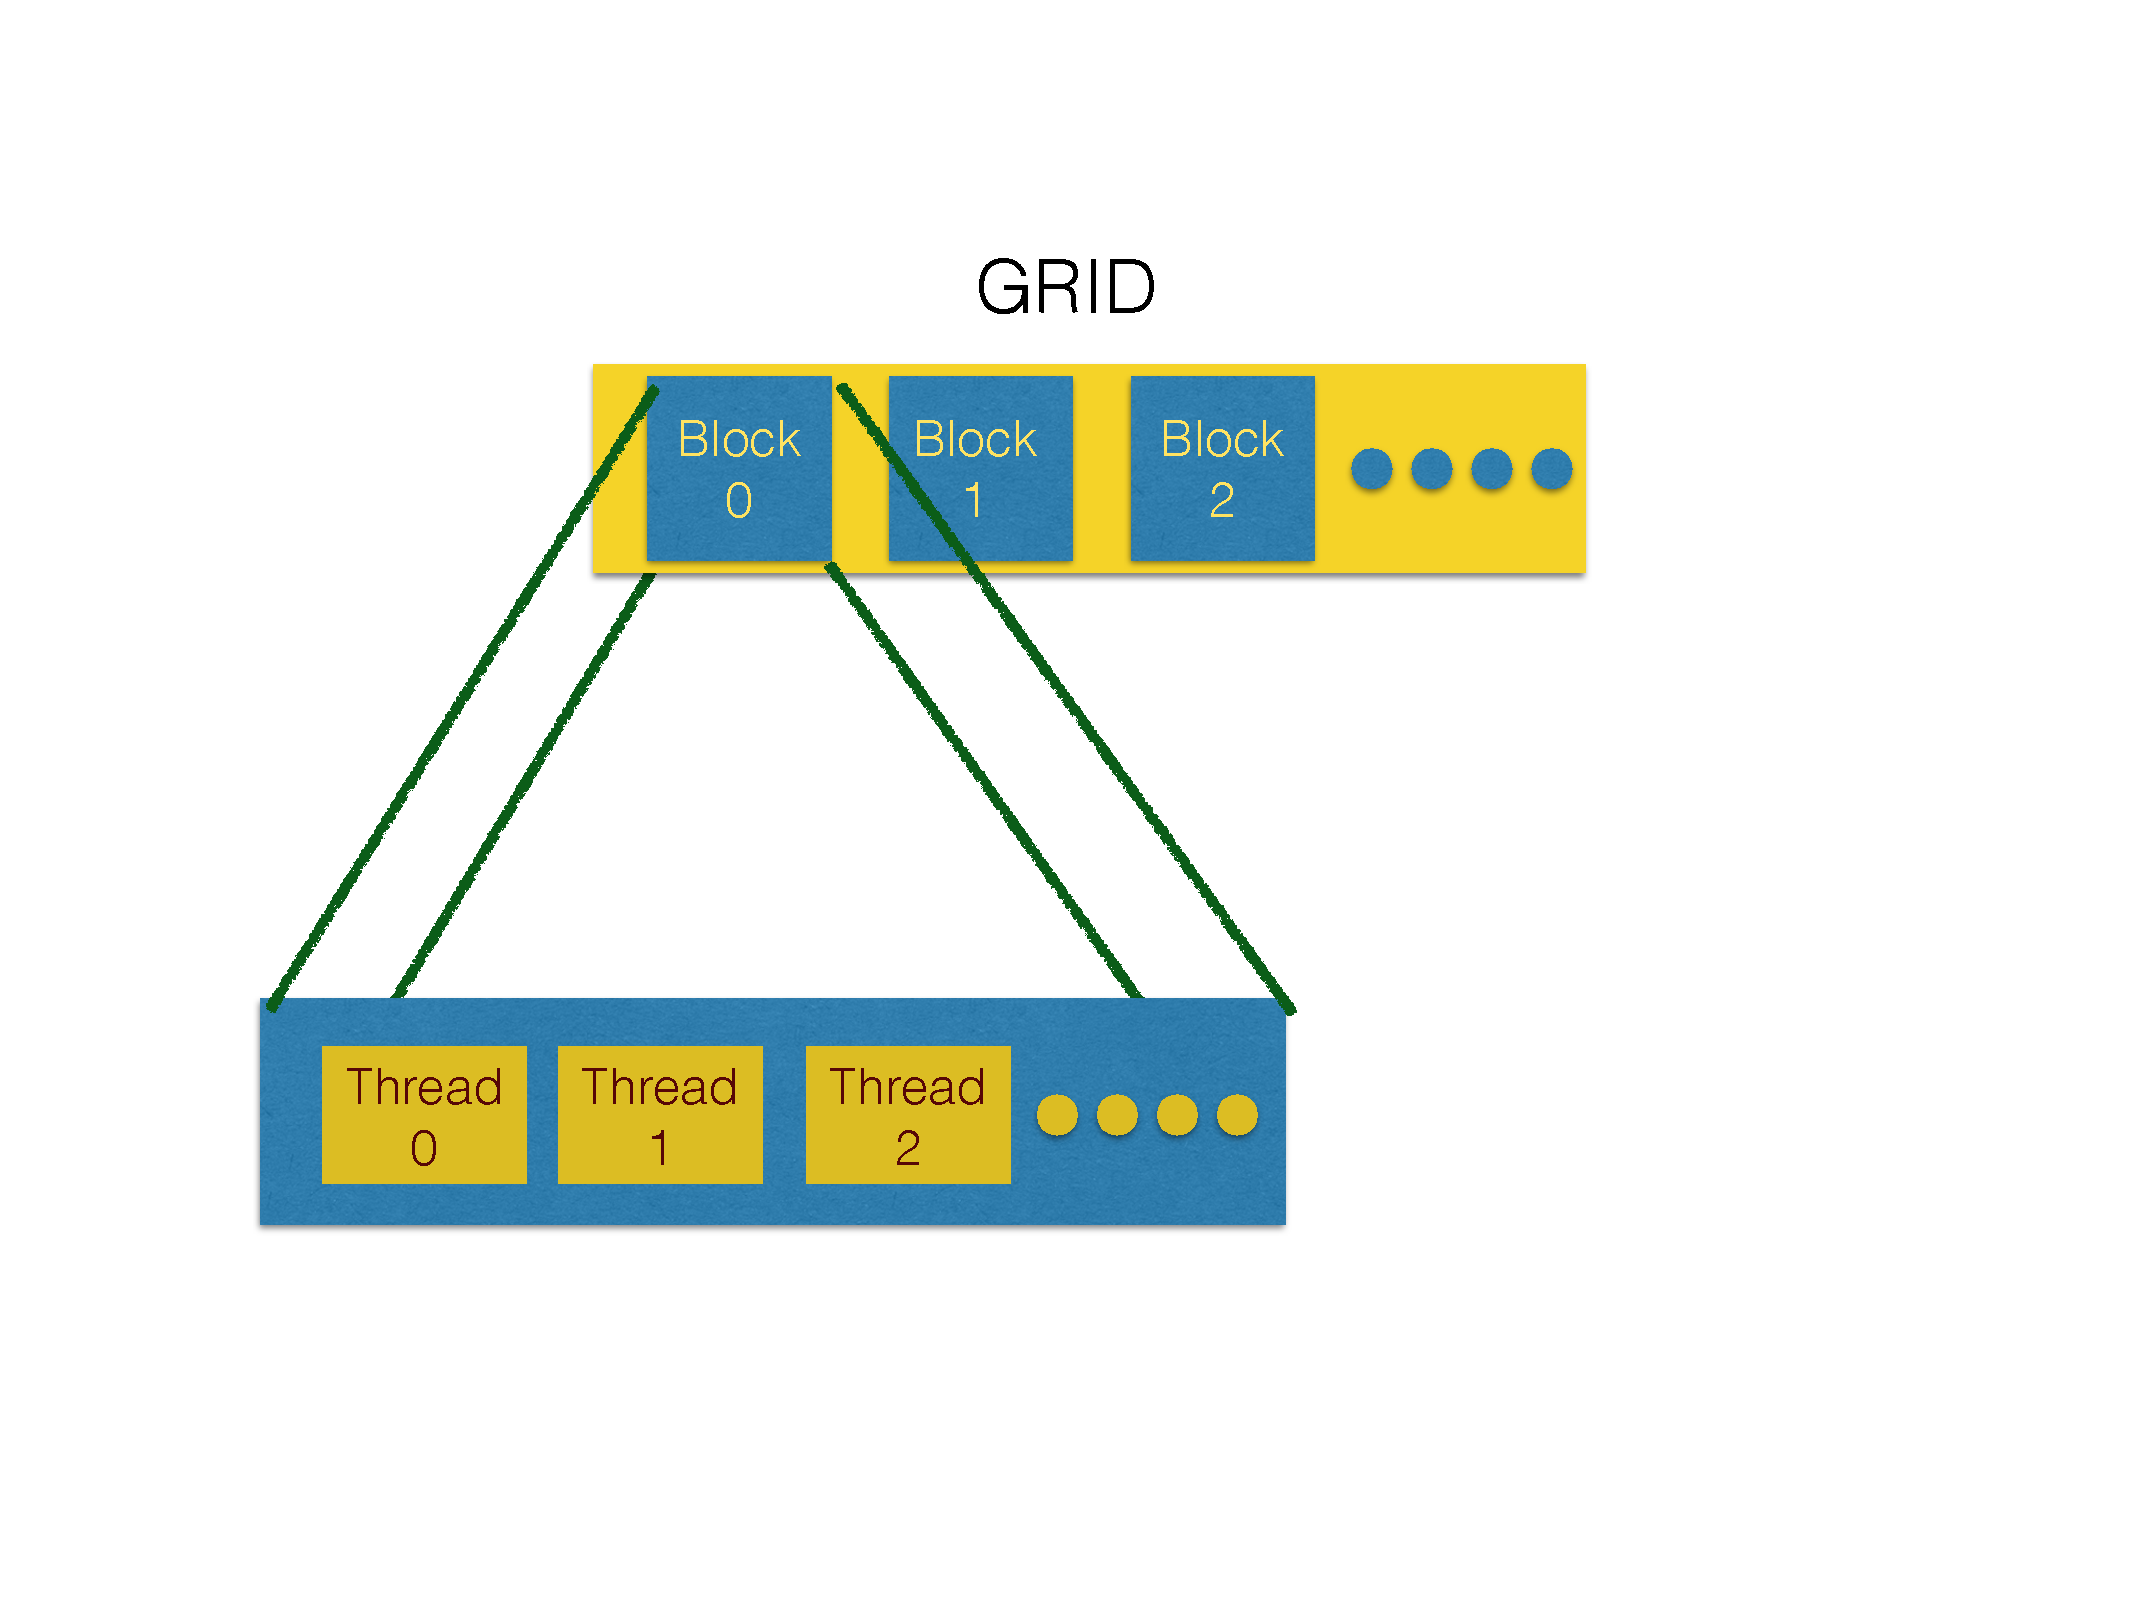
\includegraphics[width=\textwidth]{GPU.pdf}
        \caption{This figure represents the one-dimensional indexing based architecture for both threads and blocks}
        \centering
\end{figure}

\subsection*{Configuration}
Following are the hardware details of the machine used for experimentation
\begin{itemize}
    \item GPU: NVIDIA GeForce GTX 760 2GB
    \item Maximum number of threads per block: 1024
\end{itemize}

Following is the configuration of threads and blocks employed in the project
\begin{align*}
        n &= \text{Number of rows}\\
        split &= \text{Number of rows assigned to a thread}\\
        required\_threads &= ceil(n/split)\\
        numBlocks &= ceil(required\_threads/threadsPerBlock)
\end{align*}


\section*{Parallelized Fold operation}
\begin{algorithm}[H]
      \begin{algorithmic}[1]
      \STATE gpu\_input\_size $\gets$ get\_size\_of\_gpu\_input(bitmat)
      \STATE split $\gets$ n/num\_chunks
      \STATE partial\_rows $\gets ((n\%split > 0) ? (n/split + 1) : (n/split))$
      \STATE partial\_size $\gets$ partial\_rows $*$ mask\_size
      \STATE memset(partial,$0$,partial\_size)
      \STATE convert\_bitmat\_to\_gpu\_input(bitmat, gpu\_input, mapping, $n$)
      \STATE cudaMalloc(d\_mapping, $n *$ sizeof(int))
      \STATE cudaMalloc(d\_input, gpu\_input\_size $*$ sizeof(unsigned char))
      \STATE cudaMalloc(d\_partial, partial\_size $*$ sizeof(unsigned char))
      \STATE cudaMemcpy(d\_mapping, mapping, $n *$ sizeof(int) , cudaMemcpyHostToDevice)
      \STATE cudaMemcpy(d\_input, gpu\_input, gpu\_input\_size $*$ sizeof(unsigned char), cudaMemcpyHostToDevice)
      \STATE cudaMemcpy(d\_partial, partial, partial\_size $*$ sizeof(unsigned char), cudaMemcpyHostToDevice)
      \STATE foldkernel$\lll$numBlocks,threadsPerBlock$\ggg$(d\_mapping, d\_input, d\_partial, n, mask\_size, split)
      \STATE cudaMemcpy(partial, d\_partial, partial\_size $*$ sizeof(unsigned char), cudaMemcpyDeviceToHost)
      \STATE memset(foldarr,0,mask\_size)
      \FOR{\texttt{(i=0; i<partial\_rows; i++)}}
            \FOR{\texttt{(j=0; j < mask\_size; j++)}}
                \STATE foldarr[$j$] $\gets$ partial[$i*$mask\_size $+j$]
            \ENDFOR
      \ENDFOR
      \end{algorithmic}
      \caption{GPU\_Fold(bitmat,n,num\_chunks, mask\_size)}
\end{algorithm}

\begin{algorithm}[H]
      \begin{algorithmic}[1]
      \STATE threadid $\gets$ blockIdx.x $*$ blockDim.x $+$ threadIdx.x
      \STATE start\_row $\gets$ threadid $*$ split
      \FOR{\texttt{(k=start\_row; k < start\_row + split; k++)}}
            \IF{$k<n$}
                \STATE data $\gets$ d\_input $+$ d\_mapping[$k$]
                \FOR{\texttt{(j=0; j < mask\_size; j++)}}
                    \STATE partial[\texttt{threadid * mask\_size + j}] $\gets $ partial[\texttt{threadid * mask\_size + j}] $\mathrel{|}$ data[$j$]
                \ENDFOR
            \ENDIF
      \ENDFOR
      \end{algorithmic}
      \caption{foldkernel(d\_mapping, d\_input, d\_partial, n, mask\_size, split))}
\end{algorithm}


\section*{Parallelized Unfold operation}

\begin{algorithm}[H]
      \begin{algorithmic}[1]
      \STATE gpu\_input\_size $\gets$ get\_size\_of\_gpu\_input(bitmat)
      \STATE convert\_bitmat\_to\_gpu\_input(bitmat, gpu\_input, mapping, $n$)
      \STATE memset(gpu\_output, 0, gpu\_output\_size)
      \STATE cudaMalloc(d\_mapping, $n *$ sizeof(int))
      \STATE cudaMalloc(d\_input, gpu\_input\_size $*$ sizeof(unsigned char))
      \STATE cudaMalloc(d\_mask, mask\_size $*$ sizeof(unsigned char))
      \STATE cudaMalloc(d\_output, gpu\_output\_size $*$ sizeof(unsigned char))
      
      \STATE cudaMemcpy(d\_mapping, mapping, $n *$ sizeof(int) , cudaMemcpyHostToDevice)
      \STATE cudaMemcpy(d\_input, gpu\_input, gpu\_input\_size $*$ sizeof(unsigned char), cudaMemcpyHostToDevice)
      \STATE cudaMemcpy(d\_mask, partial, mask\_size $*$ sizeof(unsigned char), cudaMemcpyHostToDevice)
      \STATE cudaMemcpy(d\_output, gpu\_output, sizeof(unsigned char)$*$gpu\_output\_size, cudaMemcpyHostToDevice)
      \STATE andres\_size $\gets$ gap\_size$ * 2 * $ mask\_size $+$ gap\_size $+ 1 + 1024$
      \STATE unfoldkernel$\lll$numBlocks,threadsPerBlock$\ggg$(d\_mapping, d\_input, d\_mask, d\_output, n, andres\_size)
      \STATE cudaMemcpy(gpu\_output, d\_output, gpu\_output\_size$*$sizeof(unsigned char), cudaMemcpyDeviceToHost)
      \STATE output\_bitmat $\gets$ convert\_output\_to\_bitmat(gpu\_output,n, andres\_size);
      \end{algorithmic}
      \caption{GPU\_UnFold(bitmat,n,mask\_size)}
\end{algorithm}

\begin{algorithm}[H]
      \begin{algorithmic}[1]
      \STATE row $\gets$ blockIdx.x $*$ blockDim.x $+$ threadIdx.x
      \IF{\texttt{(row < n)}}
        \IF{\texttt{(d\_mapping[row] < n)}}
            \STATE return
        \ENDIF
        \STATE data $\gets$ d\_input $+$ d\_mapping[row]
        \STATE o\_data $\gets$ d\_ouput $+$ row $*$ andres\_size
        \FOR{\texttt{(j=0; j < mask\_size; j++)}}
            \STATE o\_data[$j$] $\gets $ data[$j$] $\mathrel{\&}$ mask[$j$]
        \ENDFOR
      \ENDIF
      \end{algorithmic}
      \caption{unfoldkernel(d\_mapping, d\_input, d\_partial, n, mask\_size, split))}
\end{algorithm}

The above pseudocodes for Fold and Unfold operation on GPU do not include the complex logic for performing these operations in compressed format. However, the other framework and functions are same. This is done to keep the express the algorithm succinctly excluding the complications of compressed format. The variables used are self-explanatory and may not be declared in the pseudocode to maintain the preciseness. 

\section*{Experiments}
\begin{figure}[ht]
        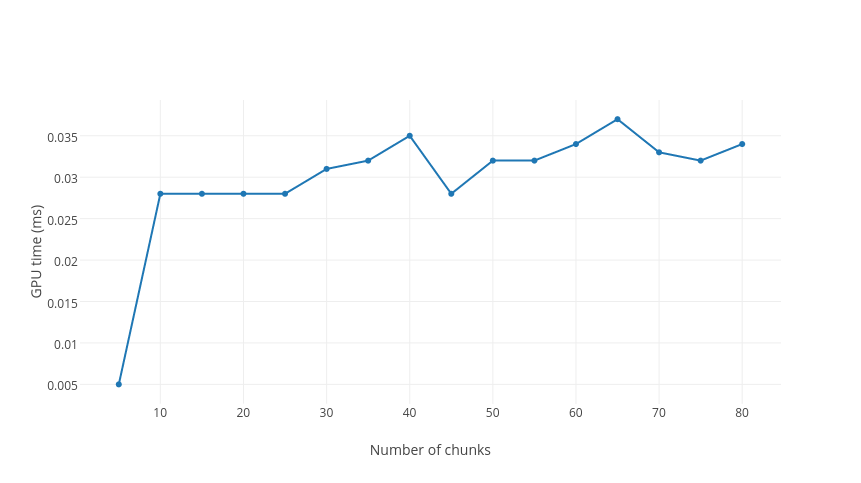
\includegraphics[width=.75\textwidth]{split_vs_gpu_time.png}
        \caption{GPU operation time vs Number of chunks}
        \centering
\end{figure}

It can be observed that changing the number of chunks (threads essentially) causes a very small effect in the time it takes for computation on GPU.

\begin{figure}[ht]
        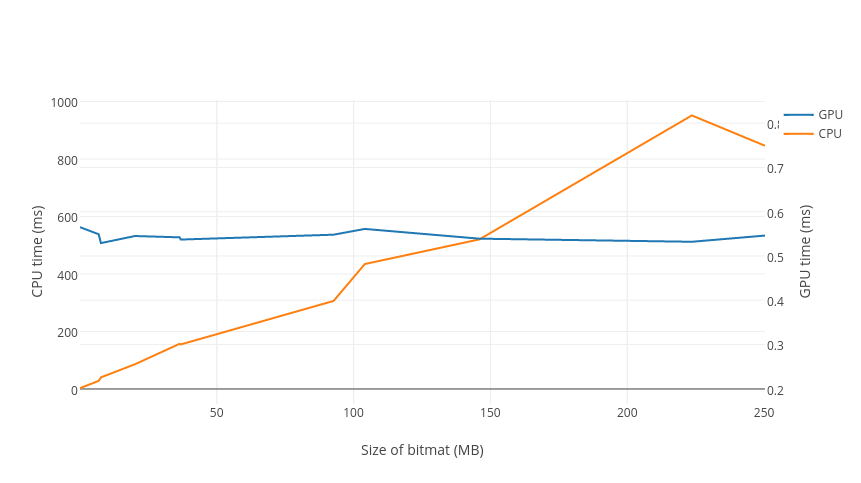
\includegraphics[width=.75\textwidth]{gpu_vs_cpu.png}
        \caption{CPU/GPU time vs size of bitmat}
        \centering
\end{figure}

Here, we observe that as the size of bitmat increases CPU time increases linearly whereas GPU time almost stays the same. This can be exploited for more efficient computation as size does not affect the GPU time computation as expected.
\pagebreak
\begin{figure}[ht]
        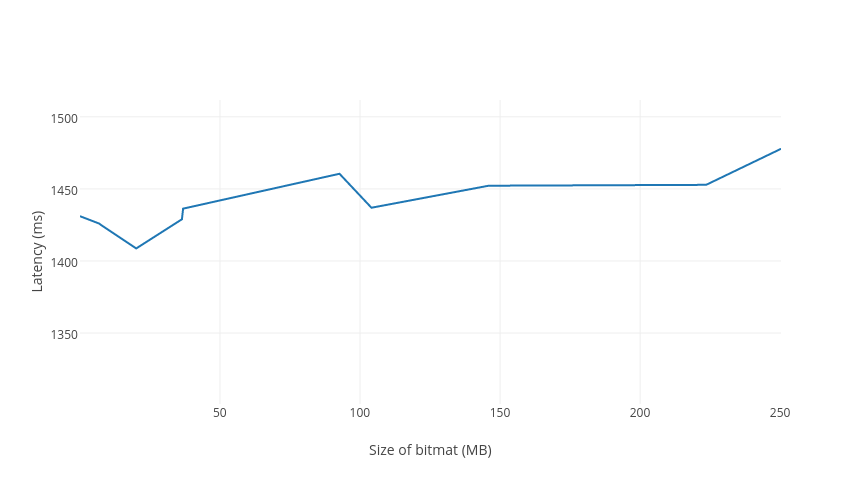
\includegraphics[width=.75\textwidth]{latency_vs_size.png}
        \caption{Latency due to data transfer vs size of bitmat}
        \centering
\end{figure}

The above plot shows an interesting phenomena. Here, it can be observed that the latency time is almost constant for any size of data. Ideally, with increasing size memory transfer should take larger time. It actually reduces the transfer overhead as apparently the size of the bitmat does not affect it.

\begin{figure}[ht]
        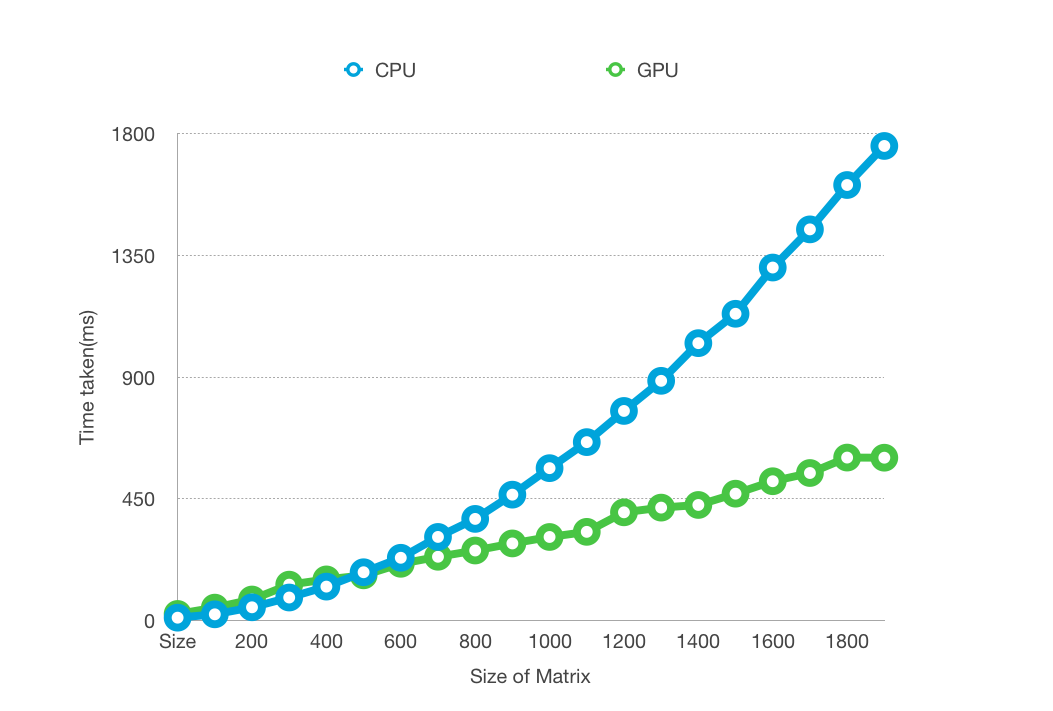
\includegraphics[width=.75\textwidth]{unfold.png}
        \caption{GPU/CPU time vs size of matrix}
        \centering
\end{figure}

This plot shows the CPU and GPU performance while performing unfold operation. It can be observed that with increasing size of matrix the GPU performs considerably better than CPU.
\pagebreak
\begin{figure}[ht]
        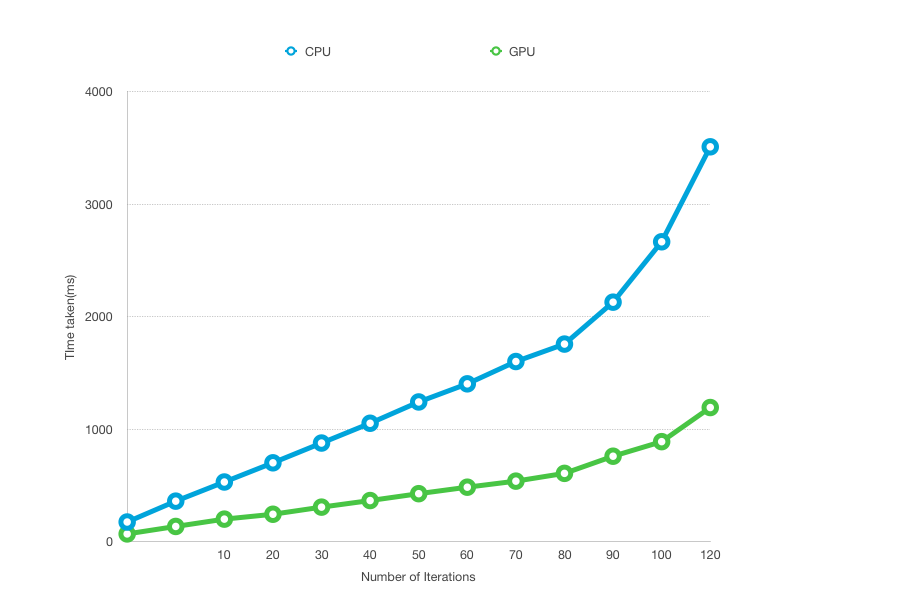
\includegraphics[width=.75\textwidth]{iter_plot.png}
        \caption{GPU/CPU time vs number of iterations}
        \centering
\end{figure}

In the above plot, we observe that once data is there in the GPU memory the unfold operation on GPU takes considerably lesser time with frequent use. The performance difference between the GPU and CPU increases with the number of iterations.

\section*{Contribution}
One of the major advantages of the above implementation for GPU is that the Fold and Unfold operations are performed in compressed format. This reduces not only the space complexity but as observed while doing operation on simulated data time complexity as well by a great amount.

Another plus point is that the implementation is compatible with the existing code base of BitMat project that performs pattern queries on these bitmats. This was also a major requirement as the existing code base has been perfected for quite a few years and it didn't make sense to rewrite the whole code for an operation. To accomplish this feat the bitmat struct was converted to a one-dimensional array with a mapping maintained as CUDA is too restrictive and doesn't support array of character arrays. In fact, one of the major bottleneck for CUDA implementation was transferring data to GPU memory and yet maintaining the compatibility.

The performance aim has been met in the above implementation especially for the unfold operation. We observe that GPU computation is significantly efficient even for small bitmats while doing unfold operation.


\section*{Future work}
The future work includes restructuring the current code as a library so that it can be imported anywhere in the existing code base. Also, currently the Unfold operation could not be tested on actual dbpedia datasets because of memory issues. So, one of the major extension is a data structure that can function in the given memory constraints and perform computation on GPU.


\end{document}
